% =================================================================
%  Weather Report -- Progress Report (CSC 475, ISMIR 2024 template)
%
%  HOW WE EDIT THIS TOGETHER
%   * Shared sections live in this file.
%   * Each person's individual status report lives in its own file
%     in sections/ so we don't get merge conflicts:
%        sections/status_jackson.tex
%        sections/status_brooklynn.tex
%        sections/status_jaiya.tex
%   * Anything in red [TODO: ...] must be filled in or deleted
%     before we submit. Search the PDF for "TODO".
%   * Build:  latexmk -pdf main.tex   (or upload the folder to Overleaf)
% =================================================================

\documentclass{article}
\usepackage[T1]{fontenc}
\usepackage[utf8]{inputenc}
\usepackage{ismir,amsmath,amssymb,cite,url}
% Remove ISMIR's CC-BY publication notice (this is a class report, not an ISMIR paper).
% Delete this line if the prof wants the notice kept.
\renewcommand{\permission}{}
\usepackage{graphicx}
\usepackage{color}
\usepackage{booktabs}
\usepackage{tikz}
\usetikzlibrary{positioning,arrows.meta,fit}

% Red placeholder for things still to fill in. Delete all before submitting.
\newcommand{\todo}[1]{\textcolor{red}{[TODO: #1]}}
% Status marks for performance-indicator tables
\newcommand{\stDone}{Done}
\newcommand{\stPart}{Partial}
\newcommand{\stNone}{Not started}

% Line numbers are only for anonymous review; not needed for this report.
% \usepackage{lineno}
% \linenumbers

\title{Weather Report: Context-Aware Playlist Generation from Photos}

\threeauthors
  {Jackson MacNeil} {University of Victoria \\ {\small\tt jacksonmacneil@uvic.ca}}
  {Brooklynn Nelson} {University of Victoria \\ {\small\tt brooklynnn@uvic.ca}}
  {Jaiya Chauhan} {University of Victoria \\ {\small\tt jaiyachauhan@uvic.ca}}

\def\authorname{J. MacNeil, B. Nelson, and J. Chauhan}

\sloppy

\begin{document}

\maketitle

% -----------------------------------------------------------------
\begin{abstract}
We present the current state of \emph{Weather Report}, a system that turns a
photo of the listener's surroundings and a target duration into a playlist
whose mood matches the scene. Photos and songs are mapped into a shared,
interpretable three-axis space: \emph{warmth}, \emph{happiness} (valence) and
\emph{energy} (arousal). On the image side, a zero-shot CLIP scorer rates each
axis with a pair of opposing text prompts and routes the warmth judgement
through an indoor/outdoor classifier. On the music side, we extract tempo,
loudness, onset rate, spectral and key/mode features with librosa, compute
CLAP zero-shot scores, and are building a hand-labelled seed set drawn from
MTG-Jamendo to train a lightweight model. This report describes the revised
design, the working components, preliminary results from prompt iteration and
tempo validation, the status of each member's performance indicators, and our
goals for the final project.
\end{abstract}

% -----------------------------------------------------------------
\section{Introduction}\label{sec:intro}

Choosing music for a walk usually means queueing songs by hand. Streaming
services recommend from listening history, but not from where the listener is
or what the day feels like. \emph{Weather Report} takes the opposite approach:
the user uploads a photo of their environment and a desired playlist length,
and the system returns a playlist whose mood and energy match the scene and,
where available, the actual weather.

The core design decision is that \textbf{images and songs are described on the
same scale}. Since our design specification we have reduced the planned six
dimensions to three axes, each scored from 0 to 1:
\emph{warmth} (cold, grey and stark vs.\ sunny, cozy and inviting),
\emph{happiness} (sad vs.\ joyful) and \emph{energy} (calm vs.\ lively).
Happiness and energy correspond to the valence and arousal axes of Russell's
circumplex model~\cite{russell1980circumplex}, which underpins most music
emotion research~\cite{kim2010mer,panda2023features}; warmth is our own
addition, motivated by the weather and context of the scene. Playlist
generation then becomes a nearest-neighbour search in this space under a
duration constraint.

We also revised two scope decisions. First, we do not train an LLark-scale
model~\cite{gardner2024llark}; instead, ``our own model'' is a small regressor
on top of librosa features and pretrained CLAP
embeddings~\cite{elizalde2023clap,wu2023laionclap}. Second, Spotify no longer
provides audio features, recommendations or preview clips to new developer
applications, so we analyse audio we can legally obtain (personal files,
FMA~\cite{defferrard2017fma} and MTG-Jamendo~\cite{bogdanov2019jamendo}) and
treat streaming export as a stretch goal.

% -----------------------------------------------------------------
\section{Related Work}\label{sec:related}

\textbf{Music emotion recognition.}
Most music emotion recognition (MER) work models emotion in the
valence--arousal plane~\cite{russell1980circumplex}. Surveys link perceived
emotion to audio features such as tempo, mode, loudness and
timbre~\cite{kim2010mer,panda2023features}, and DEAM provides continuous
valence/arousal annotations for benchmarking~\cite{aljanaki2017deam}. Our
feature extractor follows classic content-based MIR~\cite{tzanetakis2002genre}
using librosa~\cite{mcfee2015librosa}, with beat tracking based on dynamic
programming~\cite{ellis2007beat}. Tempo estimation is known to suffer from
metrical-level (octave) errors~\cite{gouyon2006tempo}, which we observe in our
own validation (\secref{sec:results}). Key and mode are estimated by
correlating chroma with the Krumhansl--Kessler key
profiles~\cite{krumhansl1990cognitive}, and harmonic/percussive separation by
median filtering~\cite{fitzgerald2010hpss} provides a drum-energy feature.

\textbf{Joint embeddings of media and text.}
CLIP~\cite{radford2021clip} learns a shared image--text embedding space and
enables zero-shot classification with natural-language prompts; prompt wording
strongly affects accuracy, motivating prompt ensembling and prompt
learning~\cite{zhou2022coop}. CLAP~\cite{elizalde2023clap,wu2023laionclap} and
MuLan~\cite{huang2022mulan} apply the same contrastive idea to audio and music.
LLark~\cite{gardner2024llark} connects music encoders to a large language
model; it is out of scope for us but inspired the project.

\textbf{Image--music matching and context.}
The closest prior work maps images and music into valence--arousal space and
matches them there, introducing the IMEMNet dataset~\cite{zhao2020imemnet};
MMVA extends this with CLIP image features, a music encoder and musical
captions~\cite{choi2025mmva}. We follow the same shared-space idea but use
interpretable zero-shot axes, add a warmth axis, and plan to incorporate
environmental context (time, location and weather), a direction surveyed in
contextual music recommendation~\cite{kaminskas2012contextual}. Playlist
generation and its evaluation are surveyed in~\cite{bonnin2014playlists}.

% -----------------------------------------------------------------
\section{System Overview}\label{sec:system}

\figref{fig:pipeline} shows the pipeline. Six components (C1--C6) were defined
in the design specification and are owned two per person
(\secref{sec:status}).

\begin{figure*}[t]
\centering
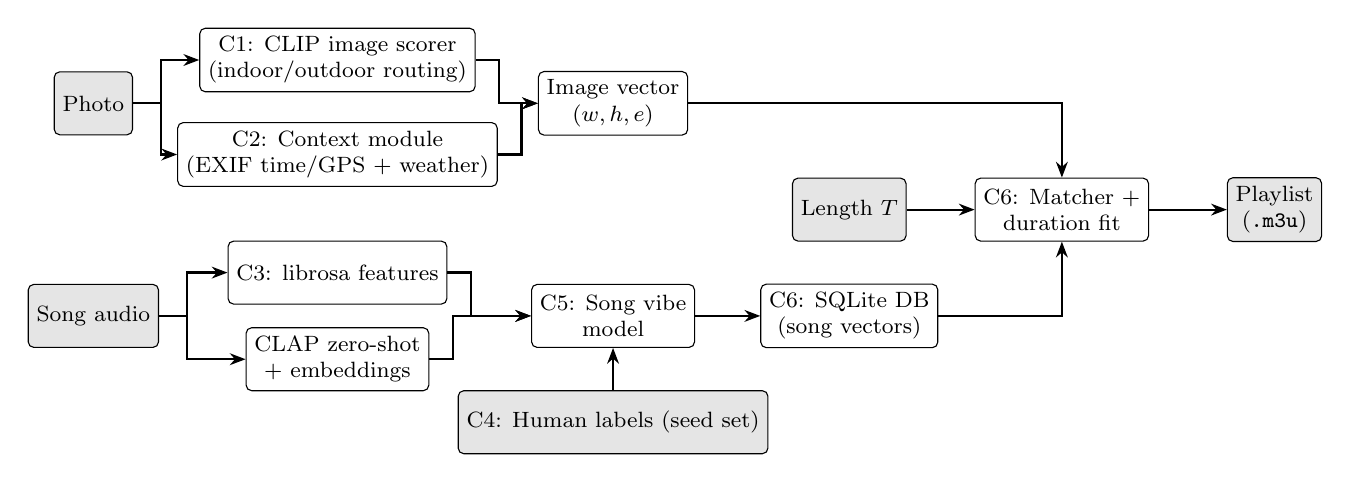
\begin{tikzpicture}[
  box/.style={draw, rounded corners=2pt, align=center, font=\footnotesize,
              minimum height=8mm, inner sep=3pt, fill=white},
  io/.style={box, fill=black!10},
  arr/.style={-{Stealth[length=2mm]}, thick}]
  % image branch (top row)
  \node[io]  (photo) at (0,0)     {Photo};
  \node[box] (clip)  at (3.1,0.55)  {C1: CLIP image scorer\\(indoor/outdoor routing)};
  \node[box] (ctx)   at (3.1,-0.65) {C2: Context module\\(EXIF time/GPS + weather)};
  \node[box] (ivec)  at (6.6,0)   {Image vector\\$(w,h,e)$};
  % audio branch (bottom row)
  \node[io]  (audio) at (0,-2.7)  {Song audio};
  \node[box] (lib)   at (3.1,-2.15) {C3: librosa features};
  \node[box] (clap)  at (3.1,-3.25) {CLAP zero-shot\\+ embeddings};
  \node[box] (model) at (6.6,-2.7)  {C5: Song vibe\\model};
  \node[io]  (labels) at (6.6,-4.05) {C4: Human labels (seed set)};
  \node[box] (db)    at (9.6,-2.7)  {C6: SQLite DB\\(song vectors)};
  % matching (right)
  \node[io]  (mins)  at (9.6,-1.35) {Length $T$};
  \node[box] (match) at (12.3,-1.35) {C6: Matcher +\\duration fit};
  \node[io]  (out)   at (15.0,-1.35) {Playlist\\(\texttt{.m3u})};
  % arrows
  \draw[arr] (photo.east) -- ++(0.35,0) |- (clip.west);
  \draw[arr] (photo.east) -- ++(0.35,0) |- (ctx.west);
  \draw[arr] (clip.east) -- ++(0.3,0) |- (ivec.west);
  \draw[arr] (ctx.east)  -- ++(0.3,0) |- (ivec.west);
  \draw[arr] (audio.east) -- ++(0.35,0) |- (lib.west);
  \draw[arr] (audio.east) -- ++(0.35,0) |- (clap.west);
  \draw[arr] (lib.east)  -- ++(0.3,0) |- (model.west);
  \draw[arr] (clap.east) -- ++(0.3,0) |- (model.west);
  \draw[arr] (labels) -- (model);
  \draw[arr] (model) -- (db);
  \draw[arr] (ivec.east) -| (match.north);
  \draw[arr] (db.east) -| (match.south);
  \draw[arr] (mins) -- (match);
  \draw[arr] (match) -- (out);
\end{tikzpicture}
\caption{The \emph{Weather Report} pipeline. Grey boxes are inputs/outputs.
Photos and songs are both mapped to a warmth/happiness/energy vector and matched
in that shared space.}
\label{fig:pipeline}
\end{figure*}

All code is written in Python~3.11 using \texttt{open\_clip}, \texttt{laion\_clap},
\texttt{librosa}, \texttt{scikit-learn} and SQLite. Components communicate
through a shared output format: a dictionary with keys \emph{warmth},
\emph{happy} and \emph{energy}, each a float in $[0,1]$. The image scorer
(\texttt{image\_to\_vector}) and the CLAP scorer (\texttt{song\_to\_vector})
already return this format; the librosa extractor (\texttt{extract\_features})
returns raw features that the song model maps into it.
\todo{Jackson: replace with the final interface list from D3.}

% -----------------------------------------------------------------
\section{Methods}\label{sec:methods}

\subsection{Zero-Shot Image Scoring (C1)}\label{sec:clip}

We use CLIP (ViT-B/32, LAION-2B weights) zero-shot. The photo and each text
prompt are embedded and compared by cosine similarity. Each axis is defined by
a pair of opposing caption-style prompts, e.g.\ ``a photo of a sad, lonely
moment'' vs.\ ``a photo of a happy, joyful moment'', and the axis score is the
softmax probability of the positive prompt within that pair. Scoring each pair
separately, rather than one softmax over all prompts, lets a photo be both
happy \emph{and} calm. A temperature (scale) factor controls how extreme the
scores are: CLIP's default of 100 produced near-binary outputs, so we use 25
for the mood axes.

Warmth proved hardest (\secref{sec:results}). Prompts about colour
temperature mistook a blue-sky beach for ``cold'', while prompts about weather
cannot judge indoor scenes. We therefore first classify the photo as indoor or
outdoor (with a sharper scale of 50). Outdoor photos are scored with weather
prompts (``cloudy, rainy day'' vs.\ ``clear, sunny day''); indoor photos with
colour/coziness prompts (``cold and stark, with blue and grey colours'' vs.\
``warm and cozy, with soft colours and light'').

\subsection{Audio Features (C3)}\label{sec:librosa}

The extractor loads each file at 22.05\,kHz mono and computes features grouped
by the axis they are expected to inform: \emph{energy} -- tempo (beat
tracking~\cite{ellis2007beat}), mean RMS loudness (dB) and onset rate (onsets/s);
\emph{warmth} -- spectral centroid (``brightness''), share of power in the
100--800\,Hz band and spectral flatness (``noisiness''); \emph{happiness} --
mode and mode strength, computed by correlating the song's average chroma
vector with all twelve rotations of the Krumhansl--Kessler major and minor key
profiles~\cite{krumhansl1990cognitive}; mode strength is the best major
correlation minus the best minor correlation, so positive values lean major.
\todo{Jaiya: add any features added since (MFCCs, duration, HPSS ratio).}

\subsection{CLAP Scoring and Song Model (C4, C5)}\label{sec:clap}

CLAP~\cite{wu2023laionclap} scores songs zero-shot with the same pairwise
prompt scoring as the image side, using audio prompts such as ``a sad and
melancholic song'' vs.\ ``a happy and cheerful song'' (scale 20). This is our
untrained baseline (System~A). Systems~B and~C will regress human labels from
librosa features alone and from librosa features plus the 512-dimensional CLAP
embedding (reduced with PCA), using ridge regression, random forests and a
small MLP. Labels are collected on MTG-Jamendo tracks, whose mood/theme tags
serve as a sanity check. \todo{Brooklynn: labelling protocol, scale (currently
Low/Mid/High), number of songs labelled, rater agreement.}

\subsection{Database and Playlist Assembly (C6)}\label{sec:db}

A shared SQLite schema stores songs, audio features, CLAP embeddings, human
ratings (with a consensus view), model scores per system and generated
playlists. Given a photo's vector and a target length, the assembler ranks
songs by Euclidean distance between the photo and song vectors and adds the
closest songs until the total length is within 3 minutes of the target.
\todo{Jaiya: update once the assembler is implemented; note schema migration
from six to three axes.}

% -----------------------------------------------------------------
\section{Preliminary Results}\label{sec:results}

\subsection{Image Scorer}

\todo{Jackson: image scorer results table on the photo test set (D5), with a
short discussion. Development-photo observations so far: the foggy forest
scores low on all three axes, the party and pub score high on happiness and
energy, the overcast harbour lands near the middle, and the night-time backyard
party is the one borderline indoor/outdoor case.}

\textbf{Prompt iteration for warmth.} \tabref{tab:warmth} summarises how the
warmth axis evolved. Colour prompts called the sunny beach cold (0.21);
``cozy'' prompts favoured indoor scenes and pushed every outdoor photo cold;
light-only prompts (``dark and gloomy'' vs.\ ``bright and clear'') rated every
photo except the fog above 0.8. Averaging the scores of two prompt pairs widened the spread, and
weather prompts plus indoor/outdoor routing gave the ordering closest to our
judgement. Earlier, single-word prompts (``warm'', ``sad'') and prompts mixing
axes (``happy, chill or relaxed'') produced confounded scores.

\begin{table}[t]
\centering\footnotesize
\setlength{\tabcolsep}{3pt}
\begin{tabular}{@{}lccccc@{}}
\toprule
Warmth prompt pair & Beach & Party & Pub & Harb. & Fog \\
\midrule
Colour (blue/grey vs.\ golden) & 0.21 & 0.80 & 0.54 & 0.58 & 0.01 \\
Stark vs.\ cozy/comforting     & 0.26 & 0.35 & 0.46 & 0.24 & 0.20 \\
Dark/gloomy vs.\ bright/clear  & 0.92 & 0.92 & 0.81 & 0.87 & 0.12 \\
Mean of colour + feeling       & 0.34 & 0.71 & 0.49 & 0.50 & 0.10 \\
Cloudy/rainy vs.\ clear/sunny  & 0.93 & 0.78 & 0.50 & 0.65 & 0.08 \\
Indoor/outdoor routed (final) & 0.93 & 0.78 & 0.64 & 0.65 & 0.08 \\
\bottomrule
\end{tabular}
\caption{Warmth scores for different prompt designs.}
\label{tab:warmth}
\end{table}

\subsection{Audio Features and Tempo Validation}

\tabref{tab:audio} shows features for two contrasting songs. The rock track is
faster, has more onsets per second and is brighter; the ballad concentrates
more power in the 100--800\,Hz ``body'' band and has a stronger major-mode
score. Tempo, however, is unreliable on slow, syncopated songs: for
\emph{Superpowers} (Daniel Caesar), librosa estimated 107.7\,BPM and
Tunebat (also algorithmic) reported 107\,BPM, whereas a hand-tapped estimate
and the Hooktheory transcription both give 80\,BPM. The ratio of about 4/3
is a metrical-level error that a simple octave fold cannot correct, so tempo
will be one of several energy cues rather than the main one.
\todo{Jaiya: full 20-song tempo validation table (D5).}

\begin{table}[t]
\centering\footnotesize
\begin{tabular}{@{}lcc@{}}
\toprule
Feature & \emph{Sex on Fire} & \emph{Fake Plastic Trees} \\
\midrule
Tempo (BPM)            & 152.0 & 73.8 \\
Loudness (dB, mean RMS) & $-15.1$ & $-16.5$ \\
Onset rate (1/s)       & 3.25 & 2.36 \\
Spectral centroid (Hz) & 2263 & 1625 \\
100--800\,Hz power share & 0.41 & 0.73 \\
Spectral flatness      & 0.018 & 0.010 \\
Mode / strength $m$    & major / 0.03 & major / 0.28 \\
\bottomrule
\end{tabular}
\caption{librosa features for two example songs.}
\label{tab:audio}
\end{table}

\todo{Brooklynn: CLAP zero-shot results on the labelled MTG-Jamendo songs
(e.g., agreement between CLAP Low/Mid/High and our labels).}

% -----------------------------------------------------------------
\section{Individual Status Reports}\label{sec:status}

Status: \stDone{} = complete; \stPart{} = started, not complete;
\stNone{} = not yet started.

% ----------------------------------------------------------------
% Individual status report -- Jackson MacNeil
% Components: C1 (CLIP image scorer), C2 (context module)
% ----------------------------------------------------------------
\subsection{Jackson MacNeil}\label{sec:status_jackson}

\begin{table}[h]
\centering\footnotesize
\begin{tabular}{@{}llp{0.5\columnwidth}l@{}}
\toprule
ID & Tier & Performance indicator & Status \\
\midrule
D1 & Basic    & Run CLIP locally; photo--prompt similarity & \stDone \\
D2 & Basic    & Prompt sets per axis; 0--1 vector per photo & \stDone \\
D3 & Basic    & Shared interfaces between components & \stPart \\
D4 & Basic    & Stub pipeline end to end on fake data & \stNone \\
D5 & Expected & 30--50 photo test set; correlation with team ratings & \stPart \\
D6 & Expected & Weather/time context (EXIF + Open-Meteo) & \stPart \\
D7 & Expected & Single command: photo + length $\rightarrow$ playlist & \stNone \\
D8 & Advanced & Compare prompt strategies and CLIP model sizes & \stPart \\
D9 & Advanced & Listening study, 8--10 participants & \stNone \\
\bottomrule
\end{tabular}
\caption{Jackson MacNeil -- performance indicators.}
\label{tab:pi_jackson}
\end{table}

D1 and D2 are complete: \texttt{Image/scorer.py} exposes
\texttt{image\_to\_vector(path)}, which returns the three-axis vector using the
pairwise scoring and indoor/outdoor routing of \secref{sec:clip}. The design
moved from six dimensions to three after single-softmax experiments showed
that several of the original dimensions were opposite ends of the same axis
(e.g., energy and calmness). D5 is under way with six development photos; the indoor/outdoor classifier (part of D6) is working,
while EXIF and weather lookup are next. D8 is partly covered by the prompt
comparison in \tabref{tab:warmth}. Remaining work: formalise the interfaces
(D3), build the stub pipeline (D4), finish the photo test set and correlation
(D5), add EXIF/weather context (D6), and connect everything into one
command (D7).
\todo{Jackson: update statuses and wording before submission.}

% ----------------------------------------------------------------
% Individual status report -- Brooklynn Nelson
% Components: C4 (labelling protocol/tool/seed set), C5 (song model + CLAP)
% Fill in the Status column (\stDone, \stPart, \stNone) and the paragraph.
% ----------------------------------------------------------------
\subsection{Brooklynn Nelson}\label{sec:status_brooklynn}

\begin{table}[h]
\centering\footnotesize
\begin{tabular}{@{}llp{0.5\columnwidth}l@{}}
\toprule
ID & Tier & Performance indicator & Status \\
\midrule
D1 & Basic    & Labelling protocol with rating scale and example songs & \todo{} \\
D2 & Basic    & Labelling tool that plays a clip and saves ratings & \todo{} \\
D3 & Basic    & CLAP zero-shot scores and embeddings for every song & \todo{} \\
D5 & Expected & $\sim$100-song seed set; coordinate labelling by all 3 & \todo{} \\
D6 & Expected & Model ratings vs.\ group ratings & \todo{} \\
D7 & Expected & Compare Systems A, B and C & \todo{} \\
D8 & Expected & Compare ridge, random forest, MLP; feature importance & \todo{} \\
D9 & Advanced & Train on a large dataset; compare with LLark & \todo{} \\
\bottomrule
\end{tabular}
\caption{Brooklynn Nelson -- performance indicators.}
\label{tab:pi_brooklynn}
\end{table}

\todo{Brooklynn: describe progress in your own words. Current repo state:
\texttt{Song/song\_scorer.py} computes CLAP zero-shot scores on the three axes
(scale 20, adjusted energy prompt); \texttt{Song/labeled\_test\_songs.csv}
holds the first eight MTG-Jamendo tracks labelled Low/Mid/High on energy,
happiness and warmth. Add what is done, what is left, and what you learned.}

% ----------------------------------------------------------------
% Individual status report -- Jaiya Chauhan
% Components: C3 (librosa feature extractor), C6 (database + playlist assembler)
% Fill in the Status column (\stDone, \stPart, \stNone) and the paragraph.
% ----------------------------------------------------------------
\subsection{Jaiya Chauhan}\label{sec:status_jaiya}

\begin{table}[h]
\centering\footnotesize
\begin{tabular}{@{}llp{0.5\columnwidth}l@{}}
\toprule
ID & Tier & Performance indicator & Status \\
\midrule
D1 & Basic    & librosa: tempo, loudness, key/mode, spectral, MFCCs, duration & \todo{} \\
D2 & Basic    & SQLite schema; store features for the seed set & \todo{} \\
D3 & Basic    & Rank songs by similarity to the photo vector & \todo{} \\
D4 & Basic    & Fit total length within $\pm$3 min; \texttt{.m3u} export & \todo{} \\
D5 & Expected & Validate tempo vs.\ hand-tapped BPM on 20 songs & \todo{} \\
D6 & Expected & Process a 300+ song library & \todo{} \\
D7 & Expected & UI for photo upload, length and playlist display & \todo{} \\
D8 & Expected & Playlist flow (no repeat artists, smooth energy) & \todo{} \\
D9 & Advanced & Deploy a web app; streaming export if possible & \todo{} \\
\bottomrule
\end{tabular}
\caption{Jaiya Chauhan -- performance indicators.}
\label{tab:pi_jaiya}
\end{table}

\todo{Jaiya: describe progress in your own words. Current repo state:
\texttt{Librosa/extract\_features.py} extracts tempo, loudness, onset rate,
spectral centroid, low-mid power share, spectral flatness and mode/mode
strength into \texttt{features.csv}; \texttt{Database/schema.sql} and
\texttt{db.py} define the shared SQLite database (still using the original six
dimensions). Add what is done, what is left, and what you learned.}


% -----------------------------------------------------------------
\section{Revised Timeline and Final Goals}\label{sec:plan}

The original timeline assumed six dimensions and a single labelling pass; both
changed. \tabref{tab:timeline} gives the revised plan.
\todo{All: confirm dates against the course deadline.}

\begin{table}[t]
\centering\footnotesize
\begin{tabular}{@{}lp{0.72\columnwidth}@{}}
\toprule
Week & Milestone \\
\midrule
Nov 16 & Shared interfaces + stub pipeline; DB migrated to 3 axes; ~100 seed songs labelled by all three members \\
Nov 23 & End-to-end CLI; train Systems B/C; photo test set rated; EXIF + weather context \\
Nov 30 & A/B/C comparison; playlist assembler on 300+ songs; simple UI; \texttt{.m3u} export \\
Final  & Evaluation, listening test (if time), final paper \\
\bottomrule
\end{tabular}
\caption{Revised timeline.}
\label{tab:timeline}
\end{table}

\textbf{Basic (deliverable even with delays):} a command-line tool that takes
a photo and returns a ranked list of songs from a library of at least 100
tracks, using the CLIP image scorer and CLAP zero-shot song scores.

\textbf{Expected:} the full pipeline in one command
(\texttt{python weather\_report.py photo.jpg --minutes 45}) with weather/time
context, a trained song model, a 300+ song library, duration-matched
\texttt{.m3u} output and a simple UI; evaluation of Systems A/B/C against held-out
human labels and of the image scorer against team ratings of a photo test set.

\textbf{Advanced:} a blind listening test comparing our playlists with
zero-shot and random baselines; a hosted web version; direct playlist export to
a streaming service if API access allows.

% -----------------------------------------------------------------
\section{Lessons Learned}\label{sec:lessons}

\emph{Prompt design is the model design.} Single words, mixed-axis
vocabulary and unbalanced prompt pairs all produced misleading scores;
describing what a scene \emph{looks like} worked better than naming an
abstract feeling. \emph{Every judge has blind spots.} Colour, light and
weather prompts each failed on different photos, and combining them
(by averaging or routing) helped more than tuning any single prompt.
\emph{Beware of tuning to the test set.} Moving the indoor/outdoor threshold to
fix one photo would not generalise; a larger photo test set rated by the team
is needed. \emph{Algorithms can agree and both be wrong,} as the tempo example
shows; human ground truth is essential. Finally, external APIs change: the
Spotify restrictions forced us to own the whole audio-analysis pipeline.

% -----------------------------------------------------------------
\section{AI Use Disclosure}\label{sec:ai}

We used Claude (Anthropic), an AI assistant, in preparing this report. It
produced the TikZ code for the pipeline diagram (\figref{fig:pipeline}), set up
the ISMIR \LaTeX{} template and helped with formatting the report, It was also used 
as a tutor and coding assistant while developing the image scorer. 
All system design decisions, experiments, code and reported results are the authors' own.
\todo{Brooklynn, Jaiya: add any AI tools you used for your components.}

% -----------------------------------------------------------------
\bibliography{references}

\end{document}
